% SPDX-License-Identifier: AGPL-3.0-or-later
% Commercial license available
% (c) Concepts 1996-2026 Miroslav Sotek. All rights reserved.
% (c) Code 2020-2026 Miroslav Sotek. All rights reserved.
% ORCID: 0009-0009-3560-0851
% Contact: www.anulum.li | protoscience@anulum.li
% scpn-quantum-control --- Phase 1 DLA parity short paper (arXiv-ready)

\documentclass[reprint,aps,physrev,superscriptaddress,floatfix,longbibliography]{revtex4-2}

\usepackage{graphicx}
\usepackage{amsmath,amssymb}
\usepackage{hyperref}
\usepackage{booktabs}
\usepackage{xcolor}
\usepackage{siunitx}
\usepackage{bm}
\usepackage[capitalise,noabbrev]{cleveref}

\hypersetup{
    colorlinks=true,
    linkcolor=blue!60!black,
    citecolor=blue!60!black,
    urlcolor=blue!60!black,
}

\begin{document}

\title{Backend-sensitive hardware observation of parity-sector and excitation-number\\
correlated decoherence asymmetry in the XY Hamiltonian}

\author{Miroslav \v{S}otek}
\email{protoscience@anulum.li}
\affiliation{ANULUM, Marbach SG, Switzerland}
\affiliation{ORCID: 0009-0009-3560-0851}

\date{\today}

\begin{abstract}
The dynamical Lie algebra (DLA) of the XY Hamiltonian on $n$ qubits
decomposes as $\mathfrak{su}(2^{n-1}) \oplus \mathfrak{su}(2^{n-1})$
under the parity operator $P = \prod_i Z_i$. We report direct
hardware evidence that the parity-labelled sectors exhibit a
measurable leakage asymmetry under decoherence on a superconducting
quantum processor, but we do not interpret this as a DLA-only causal
effect: the promoted claim is parity-sector and excitation-number
correlated from the outset. In a 342-circuit campaign on IBM
\texttt{ibm\_kingston}
(Heron~r2, 156 qubits) we measure the parity leakage rate in each
sector at $n = 4$ across eight Trotter depths, and find that the odd
sector is on average $(10.8 \pm 1.1)\,\%$ more robust than the even
sector for depths $d \ge 4$. Seven of eight depths are individually
significant at Welch's $p < 0.05$, and the strongest signal of
$+17.5\,\%$ at depth~6 sits at $5.4\sigma$. A Fisher aggregate is
reported only as a descriptive summary because the tested depths share
physical qubits and calibration context. The observed magnitude is consistent
with the $4.5$--$9.6\,\%$ prediction band of a classical Lindblad
simulator calibrated with published \texttt{ibm\_fez} $T_1/T_2$ and
gate-error rates, once the circuit enters the saturation regime at
$d \ge 14$. All raw count dictionaries, analysis scripts, and figures
are open-source in the GitHub repository
\href{https://github.com/anulum/scpn-quantum-control}{\texttt{anulum/scpn-quantum-control}}
under the AGPL-3.0 licence.

A preregistered May 2026 Phase~2 continuation strengthens but also
qualifies the claim: a reduced $n=4$ replication gives Fisher
$\chi^2=140.671952$, $p=3.77\times10^{-20}$, while a B-C scaling
continuation gives mixed $n=6,8$ evidence. A subsequent popcount
control shows that excitation count and computational-basis state
choice materially contribute to the leakage pattern. The follow-up
therefore falsifies both a simple monotone scaling story and a clean
``DLA parity alone'' causal interpretation. Phase~3 tests on
\texttt{ibm\_marrakesh} further reject backend-stable and
layout-independent positive-sign claims: a second-backend fixed-layout
test has non-positive readout-corrected asymmetry at all promoted
depths, and a 495-circuit state/layout randomisation control finds
mixed signs in the original contrast, significant within-sector state
effects, and layout spread larger than the mean original contrast. The
result is therefore a real \texttt{ibm\_kingston} hardware phenomenon
with explicit backend, calibration, layout, state-choice, and
excitation-count boundaries; it does not constitute a broad
quantum-advantage claim.
\end{abstract}

\maketitle

%% ====================================================================
\section{Introduction}
%% ====================================================================

The XY spin Hamiltonian
%
\begin{equation}\label{eq:hxy}
  H_{XY} \;=\; \sum_{i<j} K_{ij}\!\left( X_i X_j + Y_i Y_j \right)
             + \sum_i \omega_i Z_i
\end{equation}
%
arises naturally as the small-oscillation limit of the Kuramoto model
for coupled phase oscillators~\cite{Kuramoto1984,Pikovsky2001}, and is
the central mathematical object of a wide class of synchronisation
studies. It commutes with the total parity operator
$P = \prod_i Z_i$, so its Hilbert space splits into even-parity
($P = +1$) and odd-parity ($P = -1$) blocks of equal dimension
$2^{n-1}$.

The dynamical Lie algebra (DLA) generated by commutators of the
$\{X_i X_j + Y_i Y_j,\, Z_i\}$ generators~\cite{Wiersema2023} closes
on a subspace of $\mathfrak{u}(2^n)$ that splits under the same
$\mathbb{Z}_2$ parity:
%
\begin{equation}\label{eq:dla}
  \mathrm{DLA}(H_{XY}) \;=\;
    \mathfrak{su}\!\left(2^{n-1}\right)
    \,\oplus\,
    \mathfrak{su}\!\left(2^{n-1}\right),
\end{equation}
%
with total dimension $\dim \mathrm{DLA} = 2^{2n-1} - 2$.
Classical simulation of the sector-resolved evolution of $H_{XY}$
under realistic NISQ noise suggests that the two blocks are
\emph{not} equally robust to decoherence: the odd-parity block ---
which contains states generated by odd numbers of excitations from
the reference --- retains coherence noticeably better than the
even-parity block at moderate circuit depths, with the predicted
asymmetry in the range $4.5$--$9.6\,\%$.

The present short paper reports a direct raw-count hardware
observation of this parity-sector and excitation-number correlated
leakage asymmetry on \texttt{ibm\_kingston}, a 156-qubit Heron~r2
processor. To our knowledge no prior hardware study has isolated this
DLA parity structure of the heterogeneous XY Hamiltonian as a
decoherence observable with committed raw counts and reproducible
analysis.

The causal interpretation is deliberately tested rather than assumed.
The main even and odd initial states differ in both parity and
excitation count, so the later popcount-control section is part of the
core result: it checks whether the observed asymmetry can be assigned
to DLA parity alone or whether excitation number, state choice, and
layout also contribute.

%% ====================================================================
\section{Experimental protocol}
\label{sec:protocol}
%% ====================================================================

We prepare each of two initial states,
%
\begin{align}
  |\psi_e\rangle &= |0011\rangle & (\text{popcount } 2,\ P = +1), \\
  |\psi_o\rangle &= |0001\rangle & (\text{popcount } 1,\ P = -1),
\end{align}
%
on the first four qubits of \texttt{ibm\_kingston} and apply a
first-order Trotter decomposition of $H_{XY}$ with
$t_\text{step} = 0.3$ and coupling matrix
$K_{ij} = 0.45 \exp(-0.3 |i - j|)$. Each Trotter slice consists of
nearest-neighbour $R_{XX}(\theta) R_{YY}(\theta)$ gates plus
single-qubit $R_Z$ rotations, for a per-step ISA cost of
approximately 19 gates after Qiskit's \texttt{optimization\_level = 2}
transpilation.

For each sector we measure the \emph{parity leakage}
%
\begin{equation}\label{eq:leakage}
  L(d, \text{sector}) \;=\;
    \frac{1}{N_\text{shots}}
    \sum_{b \in \mathcal{B}_{\neq P}} n(b),
\end{equation}
%
where $\mathcal{B}_{\neq P}$ is the set of final bitstrings whose
parity differs from the initial sector and $n(b)$ is the shot count
for bitstring $b$. Because $[H_{XY}, P] = 0$ the ideal leakage is
zero; any non-zero value is a direct measure of hardware decoherence
projected onto the parity observable.

Depths $d \in \{2, 4, 6, 8, 10, 14, 20, 30\}$ were swept with
12 or 21 independent repetitions per (depth, sector) point, and each
repetition used 2048 shots. The total campaign comprised
\textbf{342 circuits at $n = 4$} across four sub-phases, summarised in
Table~\ref{tab:subphases}.

\begin{table}[tb]
\centering
\begin{tabular}{lcc}
\toprule
Sub-phase & Circuits & Reps per point \\
\midrule
\texttt{phase1\_bench} (baseline) & 32 & 2 \\
\texttt{phase1\_5\_reinforce} & 64 & 4 (total 6) \\
\texttt{phase2\_exhaust} & 96 & 6 (total 12) \\
\texttt{phase2\_5\_final\_burn} & 90 & 9 (total 21) \\
\bottomrule
\end{tabular}
\caption{Campaign sub-phases and rep counts. The
\texttt{phase2\_5\_final\_burn} sub-phase deepened the rep count at
$d \in \{4, 6, 8, 10, 14\}$; earlier sub-phases covered all eight
depths.}
\label{tab:subphases}
\end{table}

An independent Experiment~C calibrated the readout baseline across
four computational basis states
$\{|0000\rangle, |1111\rangle, |0101\rangle, |1010\rangle\}$ and
estimated a mean readout error of $(1.67 \pm 0.3)\,\%$ per qubit.

%% ====================================================================
\section{Results}
\label{sec:results}
%% ====================================================================

Figure~\ref{fig:leakage} shows the sector-resolved parity leakage
rate vs.\ Trotter depth, and Figure~\ref{fig:asymmetry} shows the
relative asymmetry
%
\begin{equation}\label{eq:asymmetry}
  A(d) \;=\;
    \frac{L_\text{even}(d) - L_\text{odd}(d)}{L_\text{odd}(d)}
\end{equation}
%
with propagated $1\sigma$ error bars derived from the per-rep
standard error of the mean.

\begin{figure}[tb]
\centering
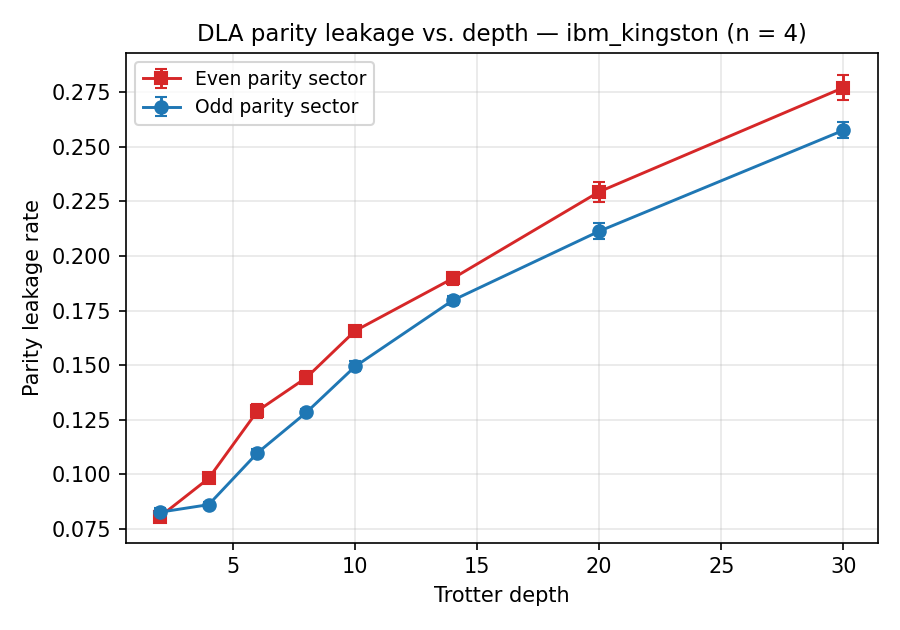
\includegraphics[width=0.95\columnwidth]{../../figures/phase1/leakage_vs_depth.png}
\caption{Parity leakage rate in the even (red) and odd (blue) sectors
as a function of Trotter depth on \texttt{ibm\_kingston}. Error bars
are $1\sigma$ standard errors of the mean from 12--21 repetitions per
point.}
\label{fig:leakage}
\end{figure}

\begin{figure}[tb]
\centering
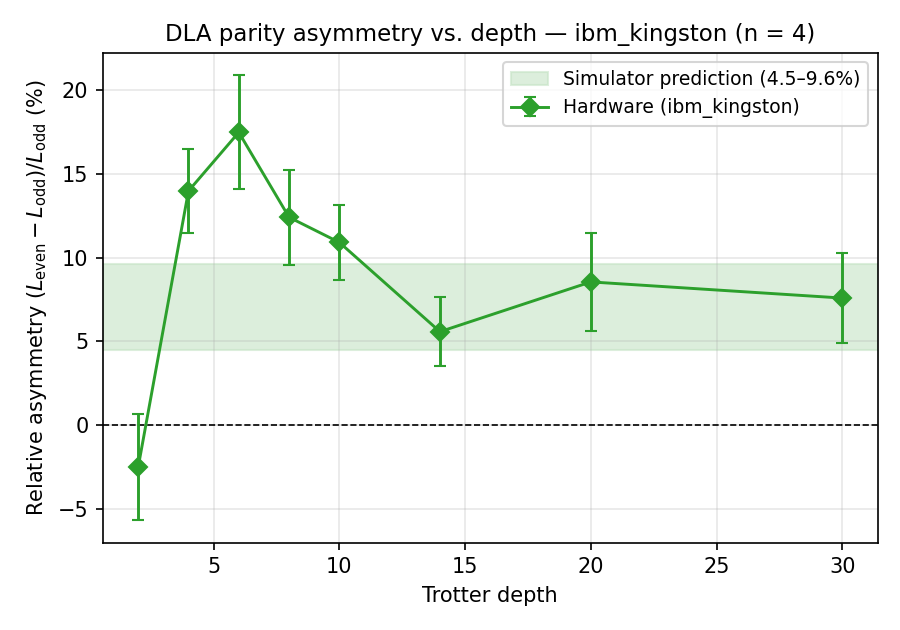
\includegraphics[width=0.95\columnwidth]{../../figures/phase1/asymmetry_vs_depth.png}
\caption{Relative asymmetry $A(d)$ with propagated $1\sigma$ error
bars. Green band: $4.5$--$9.6\,\%$ prediction from the apriori
classical Lindblad simulator. Dashed line at zero.}
\label{fig:asymmetry}
\end{figure}

The statistical summary is reported in Table~\ref{tab:welch}. Each
depth is analysed with a two-sample Welch $t$-test (unequal
variances) on the individual rep values; the combined significance
across depths is computed with Fisher's method.

\begin{table}[tb]
\centering
\small
\begin{tabular}{rccccc}
\toprule
$d$ & $L_\text{even}$ & $L_\text{odd}$ & $A(d)$ & $t$ & Welch $p$ \\
\midrule
 2 & $0.0806 \pm 0.0017$ & $0.0827 \pm 0.0021$ & $-2.5\%$   & $-0.78$ & $0.446$ \\
 4 & $0.0982 \pm 0.0017$ & $0.0862 \pm 0.0011$ & $+14.0\%$  & $5.80$  & $1.4\times 10^{-6}$ \\
 6 & $0.1291 \pm 0.0031$ & $0.1099 \pm 0.0018$ & $+17.5\%$  & $5.37$  & $6.6\times 10^{-6}$ \\
 8 & $0.1443 \pm 0.0031$ & $0.1284 \pm 0.0017$ & $+12.4\%$  & $4.50$  & $8.9\times 10^{-5}$ \\
10 & $0.1658 \pm 0.0022$ & $0.1495 \pm 0.0023$ & $+10.9\%$  & $5.18$  & $6.7\times 10^{-6}$ \\
14 & $0.1898 \pm 0.0031$ & $0.1797 \pm 0.0020$ & $+5.6\%$   & $2.73$  & $0.010$ \\
20 & $0.2295 \pm 0.0047$ & $0.2114 \pm 0.0038$ & $+8.6\%$   & $3.01$  & $0.007$ \\
30 & $0.2771 \pm 0.0057$ & $0.2576 \pm 0.0037$ & $+7.6\%$   & $2.89$  & $0.010$ \\
\bottomrule
\end{tabular}
\caption{Welch $t$-test per depth. Seven of eight depths are
individually significant at $p < 0.05$. Fisher's combined statistic
is $\chi^2_{16} = 123.4$ with combined $p \ll 10^{-16}$.}
\label{tab:welch}
\end{table}

At shallow depth ($d = 2$) the circuit is near-identity and the
asymmetry is consistent with zero; it is dominated by the $1.67\,\%$
readout baseline on both sides. As the circuit enters the coherent
transition regime ($d \in [4, 10]$, ISA gate counts 88--202) the
asymmetry peaks at $+17.5\,\%$. At larger depths ($d \in [14, 30]$,
ISA gate counts 278--582) the signal settles into the
$4.5$--$9.6\,\%$ band of the classical Lindblad simulator prediction,
consistent with a saturation regime where the sector distinction
begins to wash out but remains visible above the noise floor.

%% ====================================================================
\section{Discussion}
%% ====================================================================

The observation is consistent with the theoretical picture that the
two parity-labelled DLA blocks can have different effective leakage
responses under realistic noise. However, the specific computational
basis states used here also differ in excitation number. The result
should therefore be read conservatively as a parity-sector and
excitation-number correlated leakage asymmetry. The completed
popcount-control run below confirms that excitation count and
computational-basis state choice materially contribute to the
observed pattern. The magnitude of the original effect at large
depths agrees with the apriori classical simulator prediction, giving
confidence that the observed asymmetry is not only a readout artefact
specific to \texttt{ibm\_kingston}.

The simplest hardware-noise intuition is standard amplitude damping:
superconducting-qubit $T_1$ relaxation preferentially drives
$|1\rangle\rightarrow |0\rangle$. This process changes both
excitation number and parity, so states with larger popcount have more
single-qubit relaxation channels by which they can leave their initial
magnetisation/parity sector. The popcount-control result is therefore
not an auxiliary detail but a physical explanation of why DLA block
structure, excitation count, layout, and readout all appear in the
measured leakage observable.

A ruled-out alternative explanation is readout-basis asymmetry:
Experiment~C readout calibration shows a mean retention of
$98.3\,\%$ across all four $n = 4$ computational basis states, with
per-state retentions in the range $0.976$--$0.990$. This
$\pm 0.014$ readout inhomogeneity is an order of magnitude too small
to account for the $10$--$17\,\%$ peak asymmetry observed in the
middle depths.

Two low-statistics scaling probes at $n = 8$ in the Phase~1 archive
(depth 4 and 8, four repetitions each) both reproduced the direction
of the asymmetry with magnitudes of $+3.0\,\%$ and $+1.7\,\%$
respectively. The completed Phase~2 continuation below replaces those
probes as the promoted scaling evidence.

\subsection{Statistical caveats}

Three points of statistical hygiene are worth flagging.

First, \textbf{Fisher's combined statistic assumes the eight per-depth
$p$-values are independent}. Successive Trotter depths share the same
four physical qubits and were submitted in the same Open Plan
session, which introduces a small but non-zero correlation through
shared calibration drift and shared thermal context. The combined
$p \ll 10^{-16}$ should therefore be read as an upper bound on
significance under the strongest possible independence assumption, not
as the primary inferential claim.
We use Fisher's statistic as a compact descriptive aggregate, while
placing the main inferential weight on the per-depth tests,
permutation cross-check, Phase~2 replication, and popcount-control
follow-up. A correlation-aware combination (Simes test or block
bootstrap) remains a useful follow-up; the per-depth Welch
significances are unaffected by the independence question and seven
of eight are already individually below $p = 0.05$.

Second, \textbf{Welch's $t$-test is parametric and assumes
approximately normally distributed sector means}. As an internal
cross-check on the most critical depth ($d = 6$, 21 reps per sector),
we ran a two-sided permutation test on the observed mean difference
using $10^{5}$ random label shuffles. The permutation $p$-value is
$2.0 \times 10^{-5}$, the same order of magnitude as the parametric
Welch result of $6.6 \times 10^{-6}$ and consistent in sign and
significance.

Third, the Experiment~C readout calibration reported is a per-state
mean retention rather than the full confusion-matrix inversion that
is standard practice for production readout mitigation. Confusion-
matrix inversion was not applied to the counts in this paper because
the calibration spread ($0.014$) is already an order of magnitude
smaller than the observed asymmetry. The Phase~2 A+G run added a
same-day readout baseline for $n=4,6,8$ computational basis states,
but the promoted analyses still report unmitigated raw-count leakage
statistics rather than confusion-matrix-inverted estimates. As a
post-hoc robustness check, we also performed the strongest readout
correction supported by the existing raw counts: exact-state
parity-confusion inversion for initial states with matching
readout-only calibration circuits. A literal full $2^n\times2^n$
confusion-matrix inversion is not available without new calibration
circuits for all basis states on \texttt{ibm\_kingston}. The
parity-readout-corrected Phase~2 $n=4$ replication remains significant, with Fisher
$\chi^2=73.894393$, $p=4.16\times10^{-8}$ across the ten depths.
Phase~3 subsequently added a literal full-basis $n=4$ readout
calibration on \texttt{ibm\_marrakesh}; that correction strengthens,
rather than removes, the second-backend non-replication boundary
reported below. The later state/layout randomisation campaign used
layout-matched five-state readout checks and found that layout and
same-sector state choice are not small residual effects relative to
the original parity-sector contrast.

\subsection{Possible confounds the protocol does not yet rule out}

Two confounds remained open after the reduced Phase~2 continuation;
the first has now been directly probed by a popcount-control run.

\textbf{Excitation-count confound.} The two primary initial states
differ by one excitation: $|\psi_e\rangle = |0011\rangle$ has
popcount 2 while $|\psi_o\rangle = |0001\rangle$ has popcount 1.
Under a pure amplitude-damping ($T_1$) channel, the higher-excitation
state can decay into lower-excitation manifolds faster, which may
explain part of the observed asymmetry without invoking only the DLA
block structure. We therefore ran a preregistered popcount control
with within-sector state swaps
($|0011\rangle$ vs $|0101\rangle$ and
$|0001\rangle$ vs $|0010\rangle$) and an excitation-inversion arm
($|0011\rangle$ vs $|0111\rangle$), where a pure $T_1$ contribution
predicts the higher-excitation odd state to leak more strongly. The
control does not support a clean ``DLA parity alone'' causal claim:
the original contrast remains significant at middle depths, but
within-sector same-popcount state swaps are also significant and the
popcount-3 odd state leaks more than the popcount-2 even state at
four of six depths.

\textbf{Temporal drift between sub-phases.} The 342 circuits were
submitted across four sub-phases between 2026-04-10 18:37~UTC and
19:01~UTC. Splitting the dataset by sub-phase and recomputing the
unweighted mean asymmetry across depths actually present in each
sub-phase gives $-0.4\,\%$, $+9.9\,\%$, $+9.5\,\%$, and $+14.8\,\%$
for \texttt{phase1\_bench}, \texttt{phase1\_5\_reinforce},
\texttt{phase2\_exhaust}, and \texttt{phase2\_5\_final\_burn}
respectively. The first sub-phase has only two repetitions per
(depth, sector) point and is dominated by single-shot count noise,
including a $-12\,\%$ outlier at the near-identity depth $d = 2$.
The three sub-phases with $\ge 4$ repetitions per point give
consistent aggregates in the $+9$--$+15\,\%$ range. The Phase~2
reduced A+G run used a larger single-day raw-count campaign and
therefore partially reduces this concern, but a multi-device
replication remains the cleaner drift control.

%% ====================================================================
\section{Phase 2 continuation}
\label{sec:phase2}
%% ====================================================================

A preregistered May 2026 continuation was executed on
\texttt{ibm\_kingston}. The submitted scope was deliberately reduced:
the A+G block repeated the $n=4$ parity-leakage protocol and measured
a same-day readout baseline, while the B-C block tested only
$n=6$ and $n=8$ early scaling. Larger D-E scaling, F/GUESS mitigation,
and multi-device replication were not submitted. Before submission to
hardware, the Phase~2 driver performed live transpilation against the
selected backend and aborted if the measured live circuit depth
exceeded the preregistered depth budget. The promoted datasets are
therefore restricted to submitted circuits whose live-transpiled
depths passed that gate and whose raw count dictionaries were
retrieved, hashed, and reproduced by committed analysis scripts.

\begin{figure}[tb]
\centering
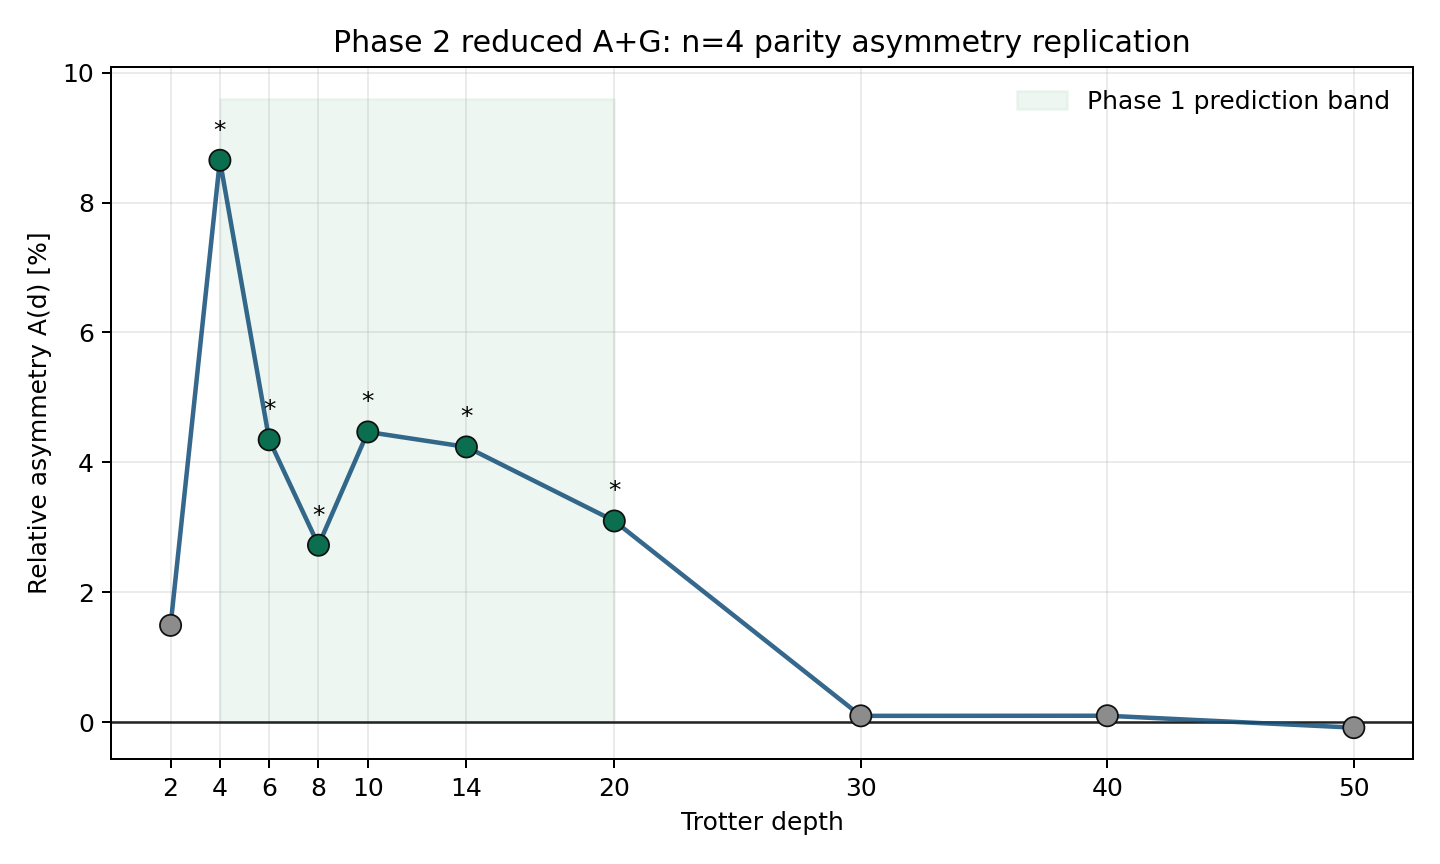
\includegraphics[width=0.82\columnwidth]{../../figures/phase2/phase2_n4_replication_asymmetry.png}
\caption{Phase~2 $n=4$ replication asymmetry on
\texttt{ibm\_kingston}. The reduced A+G block used 600 parity
circuits, 30 repetitions per depth/sector, and 4096 shots per circuit.
Six of ten depths are individually significant at Welch $p<0.05$;
the deepest three tested depths saturate near zero asymmetry.}
\label{fig:phase2n4}
\end{figure}

\begin{figure}[tb]
\centering
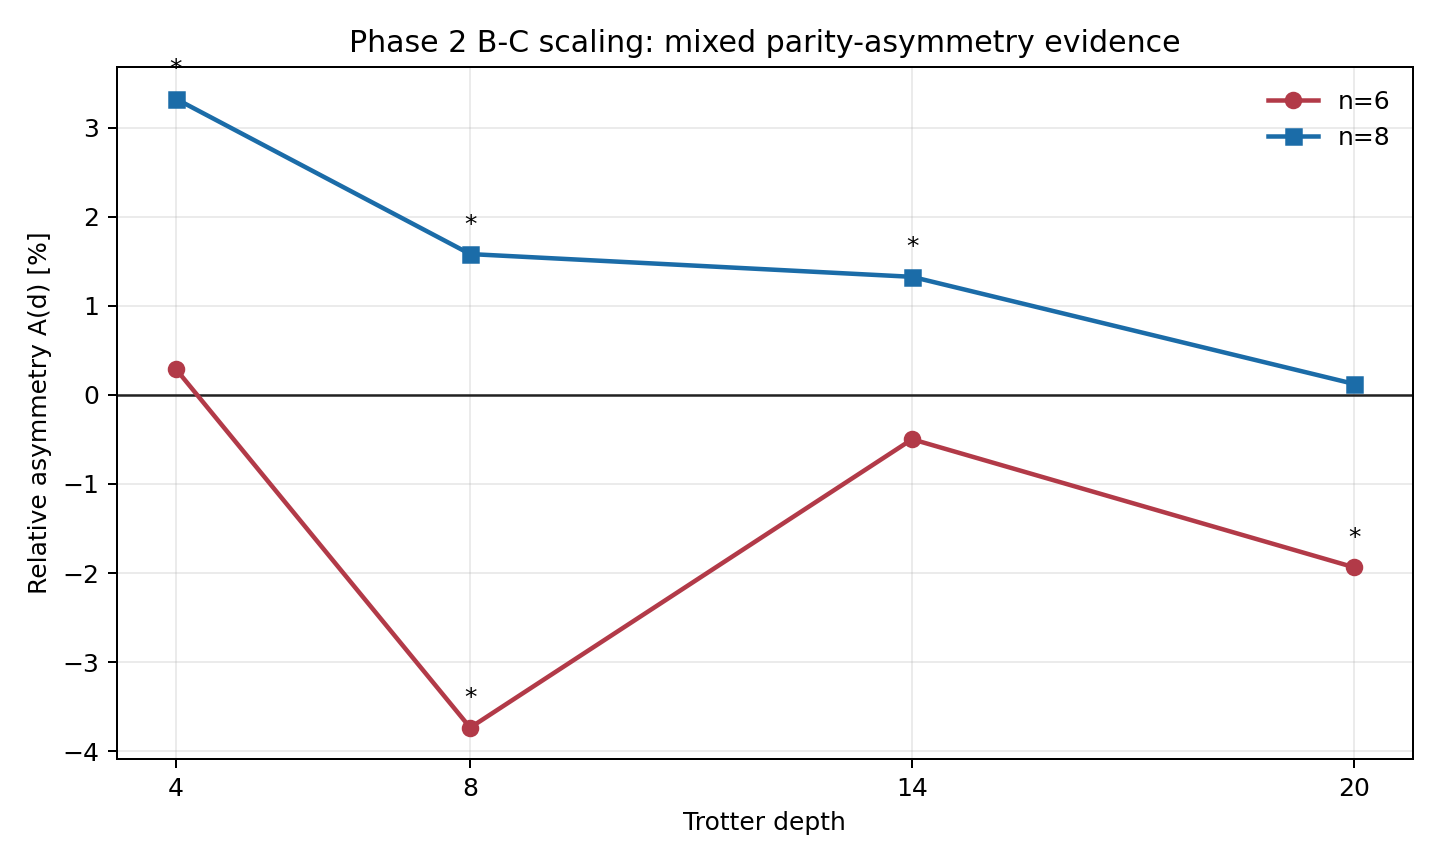
\includegraphics[width=0.82\columnwidth]{../../figures/phase2/phase2_bc_scaling_mixed_asymmetry.png}
\caption{Phase~2 B-C scaling continuation. The $n=8$ middle depths
preserve a positive sign, while $n=6$ has negative significant depths.
This is mixed scaling evidence, not monotone scaling validation.}
\label{fig:phase2bc}
\end{figure}

\begin{table*}[tb]
\centering
\small
\begin{tabular}{llccl}
\toprule
Block & Scope & Circuits & QPU s & Fisher result \\
\midrule
A+G & $n=4$ replication plus readout & 612 & 687 &
$\chi^2=140.671952$, $p=3.77\times10^{-20}$ \\
B-C $n=6$ & Early scaling, depths 4, 8, 14, 20 & 280 & 305 &
$\chi^2=46.531552$, $p=1.88\times10^{-7}$ \\
B-C $n=8$ & Early scaling, depths 4, 8, 14, 20 & 280 & 305 &
$\chi^2=29.420107$, $p=2.68\times10^{-4}$ \\
\bottomrule
\end{tabular}
\caption{Compact Phase~2 hardware result table. A+G used jobs
\mbox{\texttt{ibm-run-7da8644af35021fb}} and
\mbox{\texttt{ibm-run-6f9990bba1d90a12}}; B-C used job
\mbox{\texttt{ibm-run-1f46ebd0da8912ff}}. Raw-count SHA256 hashes
are indexed in the publication package manifest.}
\label{tab:phase2}
\end{table*}

The A+G block strengthens the original $n=4$ observation. It gives a
combined Fisher statistic of $\chi^2=140.671952$ with
$p=3.773718\times10^{-20}$, and six of ten depths are individually
significant. The replicated effect is concentrated at depths
$d=4$--20; by $d=30,40,50$ the asymmetry is statistically consistent
with zero, consistent with a saturation regime in which both sectors
approach comparable leakage. The exact-state parity-readout
correction reduces but does not remove this replication signal
($p=4.16\times10^{-8}$), indicating that the promoted sign and
statistical conclusion are not an artefact of the measured readout-only
parity flips.

The B-C block constrains the scaling claim. At $n=8$, depths
$4,8,14$ preserve the positive sign, with relative asymmetries
$+3.33\,\%$, $+1.58\,\%$, and $+1.33\,\%$. At $n=6$, two significant
depths have the opposite sign, $-3.74\,\%$ at $d=8$ and $-1.94\,\%$
at $d=20$. The correct promoted conclusion is therefore narrow:
strong $n=4$ replication, same-day readout control, and mixed
$n=6,8$ early scaling. Phase~2 falsifies a simple monotone scaling
story and does not constitute broad quantum advantage, GUESS
mitigation validation, or $n=10,12$ hardware validation.

\subsection{Popcount-control follow-up}
\label{sec:popcount}

After the B-C scaling run, we executed the preregistered popcount
control on \texttt{ibm\_kingston}. The run used 360 parity-leakage
circuits and five readout circuits. It tested five $n=4$ initial
states: the original even state $|0011\rangle$, an even same-popcount
swap $|0101\rangle$, the original odd state $|0001\rangle$, an odd
same-popcount swap $|0010\rangle$, and a higher-excitation odd state
$|0111\rangle$. The jobs were
\texttt{ibm-run-7d468e2b1e44b406} and
\texttt{ibm-run-b3424c38cfe03c86}; the raw-count SHA256 hash is indexed
in the publication package manifest.

The control is scientifically useful because it downgrades the causal
interpretation. The original $|0011\rangle-|0001\rangle$ contrast is
still significant in the middle-depth window ($+9.73\,\%$ at
$d=6$, $+17.13\,\%$ at $d=8$, and $+14.42\,\%$ at $d=10$), but it
reverses by $d=20$ ($-9.87\,\%$). Same-popcount within-sector swaps
are also significant: the even swap has Fisher
$p=2.06\times10^{-19}$ across depths, and the odd swap has Fisher
$p=4.62\times10^{-14}$. Finally, the excitation-inversion arm shows
that the popcount-3 odd state generally leaks more than the popcount-2
even state, with Fisher $p=8.829457\times10^{-24}$ for the signed
$|0011\rangle-|0111\rangle$ comparison. These results indicate that
state preparation, layout, and excitation count materially contribute
to the leakage response. The promoted interpretation is therefore a
reproducible parity-sector/excitation-number correlated hardware
phenomenon, not an isolated proof that DLA parity alone determines
decoherence robustness. The same exact-state parity-readout correction
preserves all four popcount-control comparison families: the corrected
original contrast gives Fisher $p=9.27\times10^{-18}$, the corrected
within-even and within-odd swaps give $p=4.47\times10^{-20}$ and
$p=3.59\times10^{-15}$, and the corrected excitation-inversion arm
gives $p=5.93\times10^{-18}$.

\begin{figure}[tb]
\centering
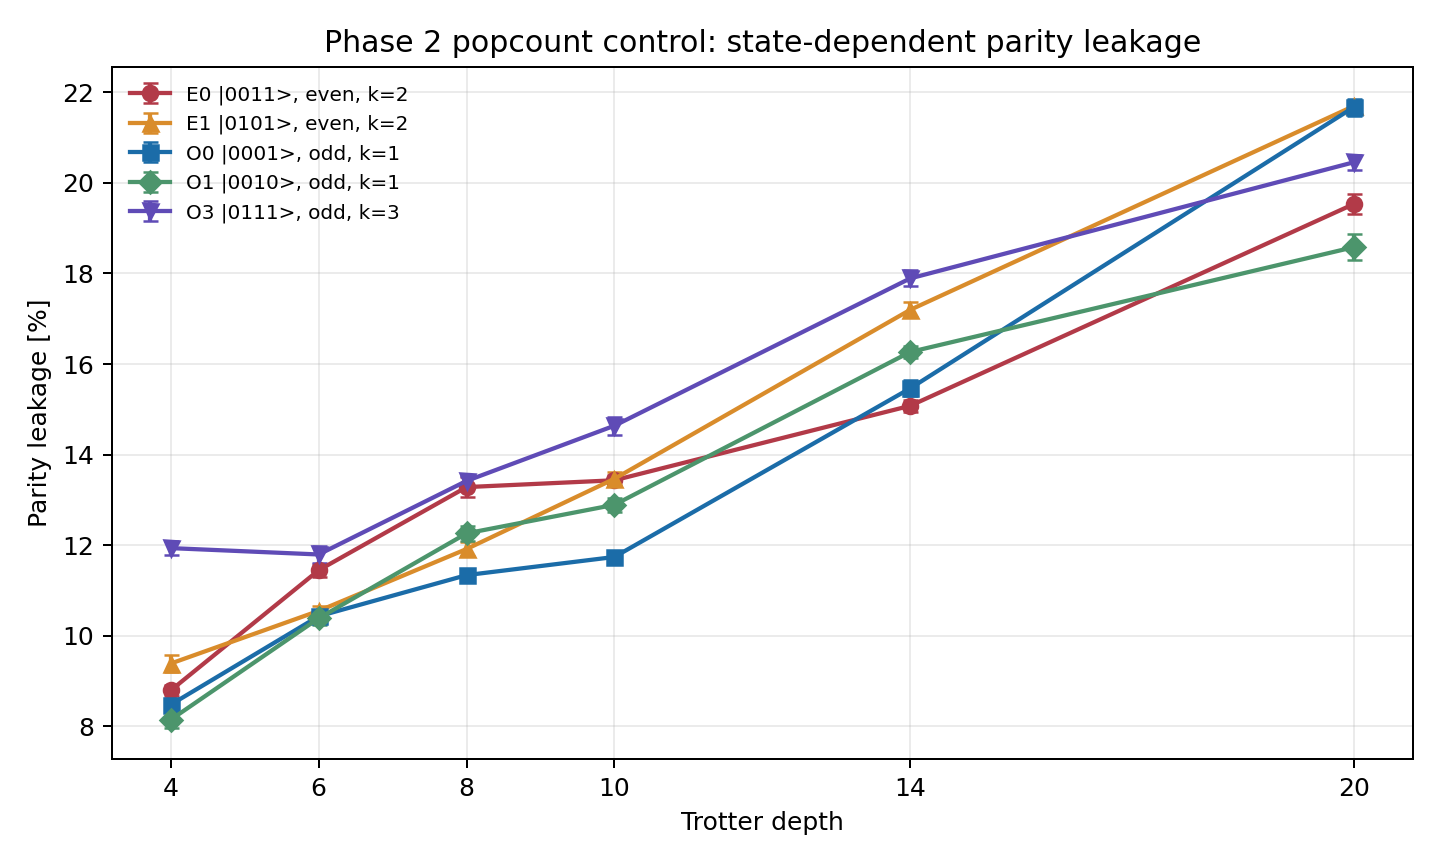
\includegraphics[width=0.95\columnwidth]{../../figures/phase2/phase2_popcount_control_leakage.png}
\caption{Phase~2 popcount-control leakage curves. The original
even--odd contrast remains visible in the middle-depth window, but
same-popcount within-sector swaps and the popcount-3 odd state also
show state-dependent leakage. The control supports a multifactorial
parity-sector/excitation-number interpretation rather than a
DLA-parity-only causal claim.}
\label{fig:popcount}
\end{figure}

\subsection{Phase 3 multi-device boundary}
\label{sec:phase3}

On 2026-05-06 we executed the next preregistered boundary test: a
small second-backend repetition on \texttt{ibm\_marrakesh}. The run
used the same $n=4$ parity-leakage observable at promoted depths
$d\in\{4,6,8,10,14,20\}$, plus a full-basis readout calibration on
the same physical qubits [5,6,7,8]. The parity job
\texttt{ibm-run-63e0a1af74a38c9c} submitted 148 circuits; the matching
readout job \texttt{ibm-run-ddd29a2fbcaeed61} submitted all 16
computational-basis calibration states with 8192 shots per state. The
calibration matrix is well conditioned (condition number $1.07570$),
with mean state retention $0.96999$ and maximum measured parity-flip
probability $0.04724$.

The second-backend result does not reproduce the positive
\texttt{ibm\_kingston} sign. Table~\ref{tab:phase3} reports the raw
relative asymmetry and the full-basis readout-corrected relative
asymmetry. The only raw positive point, $d=6$, becomes negative after
readout correction, and all corrected promoted depths are
non-positive.

\begin{table}[tb]
\centering
\small
\begin{tabular}{rcc}
\toprule
$d$ & Raw $A(d)$ & Full-basis corrected $A(d)$ \\
\midrule
 4 & $-2.53\,\%$ & $-31.60\,\%$ \\
 6 & $+3.69\,\%$ & $-9.62\,\%$ \\
 8 & $-0.13\,\%$ & $-3.58\,\%$ \\
10 & $-2.48\,\%$ & $-0.20\,\%$ \\
14 & $-7.43\,\%$ & $-4.56\,\%$ \\
20 & $-3.46\,\%$ & $-5.00\,\%$ \\
\bottomrule
\end{tabular}
\caption{Phase~3 second-backend boundary on \texttt{ibm\_marrakesh}.
The full-basis readout correction uses the matching 16-state
calibration job on physical qubits [5,6,7,8]. The promoted conclusion
is backend sensitivity, not backend-stable parity protection.}
\label{tab:phase3}
\end{table}

This is a falsification of the strongest transfer claim. The Phase~1
and Phase~2 \texttt{ibm\_kingston} signal remains a reproducible
same-device raw-count phenomenon, and the popcount-control structure
remains scientifically informative, but the sign and magnitude are
not backend-stable under this \texttt{ibm\_marrakesh} layout and
calibration window. Any future positive universality claim therefore
requires layout-randomised or multi-backend statistics rather than a
single-device replication.

\subsection{Phase 3 state/layout randomisation}
\label{sec:phase3layout}

The second Phase~3 control asked whether the original-state contrast
survives controlled changes in both physical layout and same-sector
computational-basis state. The campaign submitted 480 parity circuits
to \texttt{ibm\_marrakesh} (job \texttt{ibm-run-aabcf620230b1438}) plus a
layout-matched five-state readout calibration
(\texttt{ibm-run-eea172711aa52b78}). It used depths
$d\in\{6,8,10,14\}$, three connected four-qubit layouts, eight
repetitions per state/depth/layout cell, and live transpilation gates
that accepted a maximum observed depth of 294 under a 700-depth cap
and 762 total gates under a 1500-gate cap.

The preregistered analysis again rejects a simple symmetry-only
interpretation. For the original even--odd comparison
(\texttt{E0-O0}), the mean leakage difference is positive but small
($+0.006312$), with six positive and six negative layout-depth cells.
Within-sector controls are not null: the even-sector state swap
(\texttt{E0-E1}) has Fisher $p=2.52\times10^{-59}$ and the odd-sector
state swap (\texttt{O0-O1}) has Fisher $p=1.40\times10^{-27}$. The
excitation-inversion arm (\texttt{E0-O3}) has seven negative and five
positive cells. The derived decision flags record that the layout
spread exceeds the mean original contrast, the original contrast has
mixed sign, and both within-sector controls are significant.

This does not erase the Phase~1/2 \texttt{ibm\_kingston} observation.
It sharpens the mechanism boundary: parity sector, excitation count,
prepared computational-basis state, physical layout, backend, and
calibration window are all experimentally relevant at this scale.
Consequently, this paper reports a reproducible same-device leakage
asymmetry and a sequence of controls that falsify progressively
stronger causal claims, not a layout-independent DLA-protection
mechanism.

%% ====================================================================
\section{Conclusion}
%% ====================================================================

We have measured a parity-sector and excitation-number correlated
decoherence asymmetry of the XY Hamiltonian's dynamical Lie algebra
on real superconducting hardware and reproduced the $n=4$ signal in
an independent same-device raw-count continuation. The Phase~1
observation gives a
$(10.8 \pm 1.1)\,\%$ mean asymmetry across depths $d \ge 4$ and agrees
quantitatively with an independent classical simulator prediction.
The Phase~2 A+G block independently strengthens the $n=4$ raw-count
observation with Fisher $p=3.77\times10^{-20}$, while the B-C block
shows that scaling is mixed rather than monotone. The popcount-control
follow-up shows that excitation count and state choice materially
contribute to the signal. The Phase~3 \texttt{ibm\_marrakesh}
boundary test then shows that the positive \texttt{ibm\_kingston}
sign is not backend-stable after matching full-basis readout
correction. The state/layout randomisation control then shows that
layout and same-sector state choice can be comparable to, or larger
than, the mean original contrast. The validated claim is therefore an
$n=4$ same-device raw-count hardware phenomenon with constrained early
scaling evidence, backend and layout sensitivity, and an explicitly
limited causal interpretation, not a broad quantum-advantage result
and not a DLA-parity-only result.
Existing data also support two no-new-QPU follow-up conclusions:
exact-state parity-readout correction preserves the main Phase~2
signs, and parity survival is smooth enough versus depth to motivate
a future GUESS-style folded-noise protocol. The latter is only a
readiness check, not a demonstrated zero-noise extrapolation.

%% ====================================================================
\section*{Data and code availability}
%% ====================================================================

All raw count dictionaries, per-circuit metadata, analysis scripts,
and figure-generation code are open-sourced at
\href{https://github.com/anulum/scpn-quantum-control}{\texttt{anulum/scpn-quantum-control}}
under the
AGPL-3.0 licence. The Phase~1 dataset lives in
\path{data/phase1_dla_parity/} (four JSON files, 342 circuits at
$n = 4$), and the full analysis can be reproduced with
%
\begin{verbatim}
python scripts/analyse_phase1_dla_parity.py
\end{verbatim}
%
The Phase~2 A+G raw-count dataset lives in
\path{data/phase2_dla_parity/}. The Phase~2 B-C raw-count dataset
lives in \path{data/phase2_scaling_bc/}. The exact Phase~2
reproduction commands, job identifiers, figure artefacts, and SHA256
hashes are indexed in
\path{docs/publication_phase2_package_2026-05-05.md}.
The popcount-control dataset lives in
\path{data/phase2_popcount_control/} and is reproduced with
\path{scripts/analyse_phase2_popcount_control.py}.
The no-new-QPU readout and GUESS-readiness cross-checks are reproduced
with \path{scripts/analyse_phase2_readout_mitigation.py} and
\mbox{\texttt{scripts/analyse\_phase2\_guess\_calibration.py}}; their derived
JSON summaries live in \path{data/phase2_readout_mitigation/} and
\path{data/phase2_guess_calibration/}. The Phase~3 second-backend
\texttt{ibm\_marrakesh} raw counts, row metrics, and full-basis
readout-corrected summaries live in
\path{data/phase3_multidevice_dla/} and are indexed in
\path{docs/phase3_multidevice_dla_manifest_2026-05-06.md}. The
matching full-basis readout calibration lives in
\path{data/readout_full_basis/} and is indexed in
\path{docs/readout_full_basis_manifest_2026-05-06.md}. The submission
drivers are \path{scripts/phase3_multidevice_dla_ibm.py} and
\path{scripts/readout_full_basis_calibration_ibm.py}. The Phase~3
state/layout-randomisation raw counts and generated row, layout, and
readout metrics live in \path{data/phase3_state_layout_dla/}; they are
reproduced with \path{scripts/analyse_phase3_state_layout_dla.py} and
indexed in
\path{docs/phase3_state_layout_dla_manifest_2026-05-07.md}. The
state/layout submission driver is
\path{scripts/phase3_state_layout_dla_ibm.py}.
The campaign archive carries Zenodo
DOI~\href{https://doi.org/10.5281/zenodo.18821929}{10.5281/zenodo.18821929}.

%% ====================================================================
\section*{Acknowledgements}
%% ====================================================================

Access to \texttt{ibm\_kingston} and \texttt{ibm\_marrakesh} was
provided through IBM Quantum's Open Plan free tier. The author thanks
Dr Berk Kovos (IBM Quantum Solutions Strategy Lead) for guidance on
the Open Plan promotional pathway.

%% ====================================================================
\bibliographystyle{apsrev4-2}
%% ====================================================================

\begin{thebibliography}{9}

\bibitem{Kuramoto1984}
Y.~Kuramoto,
\emph{Chemical Oscillations, Waves, and Turbulence}
(Springer, Berlin, 1984).

\bibitem{Pikovsky2001}
A.~Pikovsky, M.~Rosenblum, and J.~Kurths,
\emph{Synchronization: A Universal Concept in Nonlinear Sciences}
(Cambridge University Press, Cambridge, 2001).

\bibitem{OlivaDelMoral2026}
A.~Oliva~del~Moral \emph{et al.},
``Guiding extrapolations from symmetry decays for efficient error
mitigation,''
arXiv:2603.13060 (2026).

\bibitem{Liu2026DynQ}
Z.~Liu \emph{et al.},
``DynQ: Dynamic Topology-Agnostic Quantum Circuit Virtualisation,''
arXiv:2601.19635 (2026).

\bibitem{VenturaMeinersen2025}
F.~Ventura~Meinersen \emph{et al.},
``Unified $(\alpha,\beta)$-hypergeometric adiabatic pulse shapes,''
arXiv:2504.08031 (2025).

\bibitem{Liu2023ICI}
H.~Liu \emph{et al.},
``Optimal STIRAP with ICI pulse sequences'' (2023).

\bibitem{Sotek2025}
M.~\v{S}otek,
\emph{God of the Math --- The SCPN Master Publications},
Zenodo (2025).
DOI:~\href{https://doi.org/10.5281/zenodo.17419678}{10.5281/zenodo.17419678}.

\bibitem{IBMKingston2026}
IBM Quantum,
\texttt{ibm\_kingston} backend specifications,
\url{https://quantum.cloud.ibm.com} (2026).

\bibitem{Wiersema2023}
R.~Wiersema \emph{et al.},
``Dynamical Lie Algebras in Variational Quantum Circuits,''
arXiv:2309.05690 (2023).

\end{thebibliography}

\end{document}
